\chapter{绪论}
随着科技的迅速发展,云计算技术已经渗透进人们生活的方方面面。云环境下数据的隐私安全问题,引起了人们的广泛关注。如何在提供高效的云服务的同时,保护用户的隐私数据不泄露以及通用的安全计算协议是当今学术研究中的热点问题。本章首先介绍云环境下的外包计算背景,以及设计隐私保护聚类方案的重要意义,然后阐述了本文的主要工作内容及创新点,最后给出了文章的整体结构。
\section{研究背景与意义}
% 直接一把子照搬开题报告!
随着现代社会数字化的不断演进,数据使用量呈指数级增加,个人和小型组织越来越 难以在内部计算机服务器上维护所有重要信息、运行大型程序和系统。为解决这些问题,云计算应运而生。自云计算在2006年被提出后,它就被认为是能够推动下一代互联网革命 的技术,并迅速成为了研究领域的热门话题\cite{sadiku2014cloud}。云计算既可以指在网络上提供的应用服务,也可以指数据中心中提供这些服务的硬件和系统软件。这些服务通常被称为软件即服务(SaaS),数据中心的硬件和软件就是我们所说的云。云计算的核心思想是,将众多用 网络连接的计算资源统一管理和调度,构成一个计算资源中心向用户提供按需服务。云计算的运行原理和基于Web的电子邮件客户端类似,允许用户访问系统的所有功能和文件,但是无需将系统的大部分内容保存在自己的计算机上。Gmail、Google Drive、TurboTax、甚至Facebook和Instagrm都是基于云的应用程序。

云计算具有诸多特点,包括可管理性,可扩展性和可用性。同时,它还具有经济、按需服务、方便、通用、多租户、灵活、稳定等特点。云计算主要提供了三种服务交付模式,分别是基础设施即服务(IaaS)、平台即服务(PaaS)、以及软件即服务(SaaS)。IaaS将计算机硬件(例如 网络存储,虚拟机,数据中心,处理器和内存)视为一种服务,无需大量资金和时间即可 提供可扩展基础架构。同时,IaaS还可以用于构建防火墙,虚拟机监控和其他安全领域\cite{manvi2014resource}。PaaS位于服务模型的中间件,以开发工具、框架、架构、程序和集成开发环境的形式提供服务。在发展的同时,PaaS还面临着诸多挑战,例如第三方关系,生命周期开发和底层基础设施安全等问题\cite{rani2014comparative}。SaaS是远程计算服务的集合,它使得第三方供应商能够远程部 署应用程序。云计算客户可以在云基础设施上通过网络获取云服务提供商的应用程序\cite{antonopoulos2010cloud}。
%\begin{figure}[htbp] 
%	\centering
%	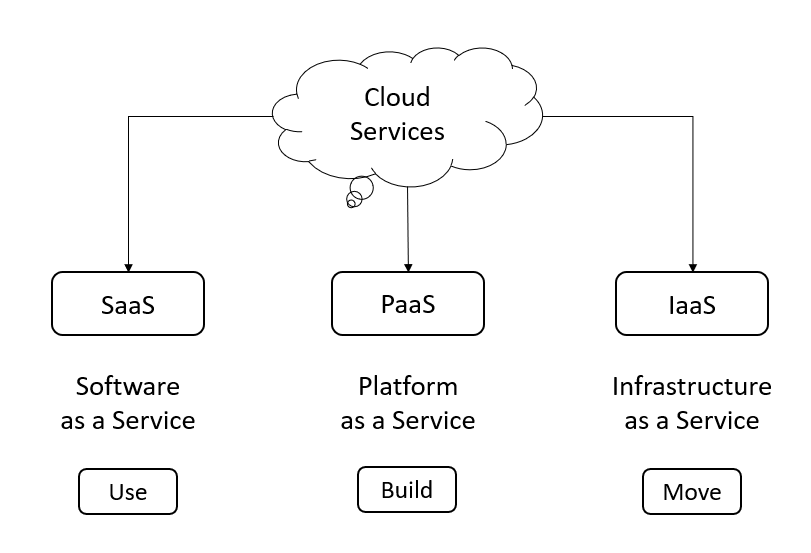
\includegraphics[width=3in]{img/cloud_model.png}%width=\linewidth
%	\caption{云服务模型}
%	\label{sys model}
%\end{figure}
近年来,随着研究的发展和设备的进步,机器学习从学术研究落地到生活的方方面面,但是大多数机器学习任务对于设备的性能要求较高,需要存储海量的数据才能取得较好的结果。大型公司有能力承担设备费用,利用机器学习的便利开展各种各样的服务,但是资源受限的小公司和个人的需求常常难以被满足。好在,云计算场景下出现了一种新的服务类型-MLaaS,即“机器学习即服务(Machine Learning as a Service)”,它使得技术可以扩展,并且价格合理\cite{ribeiro2015mlaas}。

MLaaS基本上是一组基于云的工具的总称,这些工具以一种全新的方式支持科学家和数据工作者的日常工作,它们支持协作,版本控制,并行化和其他比较复杂的任务。此外,较大的云服务供应商提供了简单明了的方法来将她们的MLaaS服务与其他工具集成,方便用户进行自动化部署以及执行机器学习任务。MLaaS包含很多种类,例如自然语言处理、图像和视频分析,计算机视觉,语音识别等等。随着机器学习技术的发展和进步,提供MLaaS的公司数量也在增加,主流的公司包括微软的Azure,谷歌的Google Cloud ML等等。在MLaaS中,海量的数据需要被上传到云计算中心,这一过程也被称之为外包计算。由于用户在数据上传后失去了对数据的完全控制,因此会更加关心隐私安全问题。同时云计算服务模型的复杂性、实时性,数据的多元异构特点以及终端资源有限,传统的数据安全隐私和隐私保护方法无法直接用来保护云计算中的大量数据\cite{hunt2018chiron}。

将一些敏感的数据进行外包以获取机器学习的结果可能会引发隐私泄漏问题,特别是在金融以及医疗领域。以医疗影像识别为例,在对数据不进行任何处理的前提下交付给云服务器进行训练,会直接造成用户隐私的泄漏,引发公众恐慌。即便是对用户的数据进行了简单的脱敏,随机处理,模型训练的中间结果也能够被恶意利用,获取信息。以k-means聚类为例,虽然原始数据经过脱敏,但是中间结果,例如聚类簇的大小,能够直接告诉我们某种特征的群体有多少人,数据的分布特点,特别有研究表明可以通过一些手段从中间结果恢复原始数据。因此,如何能够安全的进行外包计算,在维护用户数据安全隐私的同时,正确的获取外包机器学习任务的结果成为一个研究热点。

聚类(Clustering)是一种非常流行的无监督机器学习技术,它了能够将相似的输入元素划分到同一个簇(cluster)中。聚类的应用领域非常广泛,从业务分析到医疗保健等诸多领域。在许多这些应用场景中,敏感信息在被正确聚类的同时,也不应该被泄漏。此外,现在经常需要将不同来源的数据组合起来进行训练以提升分析质量,庞大的数据量对资源受限的用户带来巨大的压力,因此,通常需要将复杂的计算外包给强大的云服务器进行处理,这就要求我们设计有效隐私保护聚类方案\cite{ahmed2020k}。目前,为了保护聚类过程中输入的敏感数据的隐私,已经有了许多研究成果,涵盖各个方面。在设计隐私保护聚类协议时,通常考虑两个不同的场景。在多方计算的场景下\cite{cramer2015secure},两个及两个以上的数据所有者共同执行安全计算协议,除了输出之外的任何内容都不会泄漏给彼此,比较常见的是两方计算。同时,一些研究也会在模型设计中引入半诚实参与方(通常是服务器)来辅助计算。相对应的,另一种场景则是外包计算\cite{li2018privacy},一个或多个数据所有者将将计算(或存储)外包给其他参与方,我们假设这些参与方可以为数据所有者进行聚类而无需知道关于输入数据的任何信息。由于外包计算旨在使用外部资源,数据所有者通常不应该参与协议的执行,处于离线状态,但是这一点通常难以完全实现。值得一提的是,一些多方计算(MPC)议也可以用于外包计算场景,只需要数据所有者在多个不共谋的参与方之间秘密共享自己的数据,然后多个参与方在秘密共享的数据上执行聚类算法。但是,MPC协议是否支持外包计算很大程度上取决于协议设计,如果数据持有者需要在聚类过程中进行大量的明文计算或者在中间对数据进行解密,那就很难将协议转换到外包计算的场景。

外包计算和多方计算都各有其优势,但是对于资源受限的用户来说,外包计算则更加具有实际意义,基于外包计算的安全计算方法已有诸多研究,但是完全安全的聚类方案通常效率较低,即便是在性能较好的服务器上也需要花费难以接受的时间才能获得最终结果,效率较高的方案通常会牺牲一定的安全性,泄漏中间计算结果,例如簇大小,簇中心,这些都会导致一些隐私安全问题。因此如何设计出安全又高效的外包聚类方案值得深入研究和探索。

综上所述,本文以云计算下的外包聚类为主要应用场景,深入分析其面临的基本问题和技术难点,以设计兼具效率与安全的方案为主要目的,针对典型的聚类算法(k-means,DBSCAN)展开,提出了完善的隐私保护方案,并通过理论分析和真实数据集测试,验证所述方案的安全性,高效性和正确性。通过本文的研究,我们期望能够为资源受限的用户提供一种可行的外包聚类方法,为云服务提供商与独立用户提供合作的桥梁,使得用户能够专注于数据的挖掘分析,云服务提供商的提高资源利用率,各司其职,物尽其用,让更多人无需顾虑数据安全更加放心的享受科技进步带来的生活水平的提升。
\section{聚类中隐私保护问题综述}
本节首先介绍聚类的概念和云环境下聚类的典型应用场景,然后讨论云环境下聚类都存在哪些具体的数据安全与隐私问题,最后讨论针对上述问题目前已有的解决方案和技术手段。
\subsection{云环境下聚类综述}
本小节首先介绍云计算的基本概念和常见应用场景,然后对机器学习中的聚类技术展开介绍,最后介绍云环境下的聚类方案基本应用。
\subsubsection{云计算概述}
云计算是指一种基于互联网的按需提供计算机系统资源,特别是数据存储(云存储)和计算能力,并且无需用户自行采购、配置或管理资源的计算模式\cite{montazerolghaem2020green},其允许用户通过互联网使用分布在世界各地的服务器上的资源。云计算的部署模型通常可以分为三种,分别是公有云、私有云和混合云。公有云由第三方云服务提供商运营,使用户可以按照特定要求和业务目标安排资源部署。私有云由单个组织构建管理,以非公开的方式托管在本地,通过更强的数据控制、安全和管理功能。混合云是上述二者的结合体,使得用户既能利用公有云服务,同时保持私有云架构中常见的安全和合规功能。

云计算具有灵活性、成本低、高可靠、以及可共享等优点,带给用户巨大的便利,资源受限的用户无需关心如何部署、管理和维护IT基础设施,只需要付费即可获取想要的资源和服务。这项技术解放了用户的双手,使他们能够专注于本领域的研究与工作,提升效率。

\subsubsection{聚类算法概述}
聚类是一种无监督学习算法
\subsection{云环境下聚类中的隐私问题}
\subsection{聚类隐私保护技术手段}
\subsection{隐私保护聚类方案设计目标}
\section{研究内容和创新点}
\subsection{隐私保护外包k-means聚类方法研究}
\subsection{隐私保护DBSCAN系列研究}
\subsubsection{隐私保护DBSCAN方案}
\subsubsection{改进的隐私保护DBSCAN方案}
\subsubsection{基于DBSCAN的隐私保护层次聚类}
\section{论文的组织结构}

